% !TEX root = ../../report.tex

\clearpage
\section{PCB}\label{chapter:pcb}

While the main objective of the project is to create a MIMD system, which
essentially can be completed by FPGA design alone, everything depends on the PCB
to complete the system. It is the final step in realizing the system as a whole,
going from a theoretical dimension of design and ideas, to a physical one with
components and electricity.

The following sections have been ordered as much as possible according to which
stage in the process they occurred.

% !TEX root = ../../report.tex

\chapter{Schematics}\label{apx:schematics}

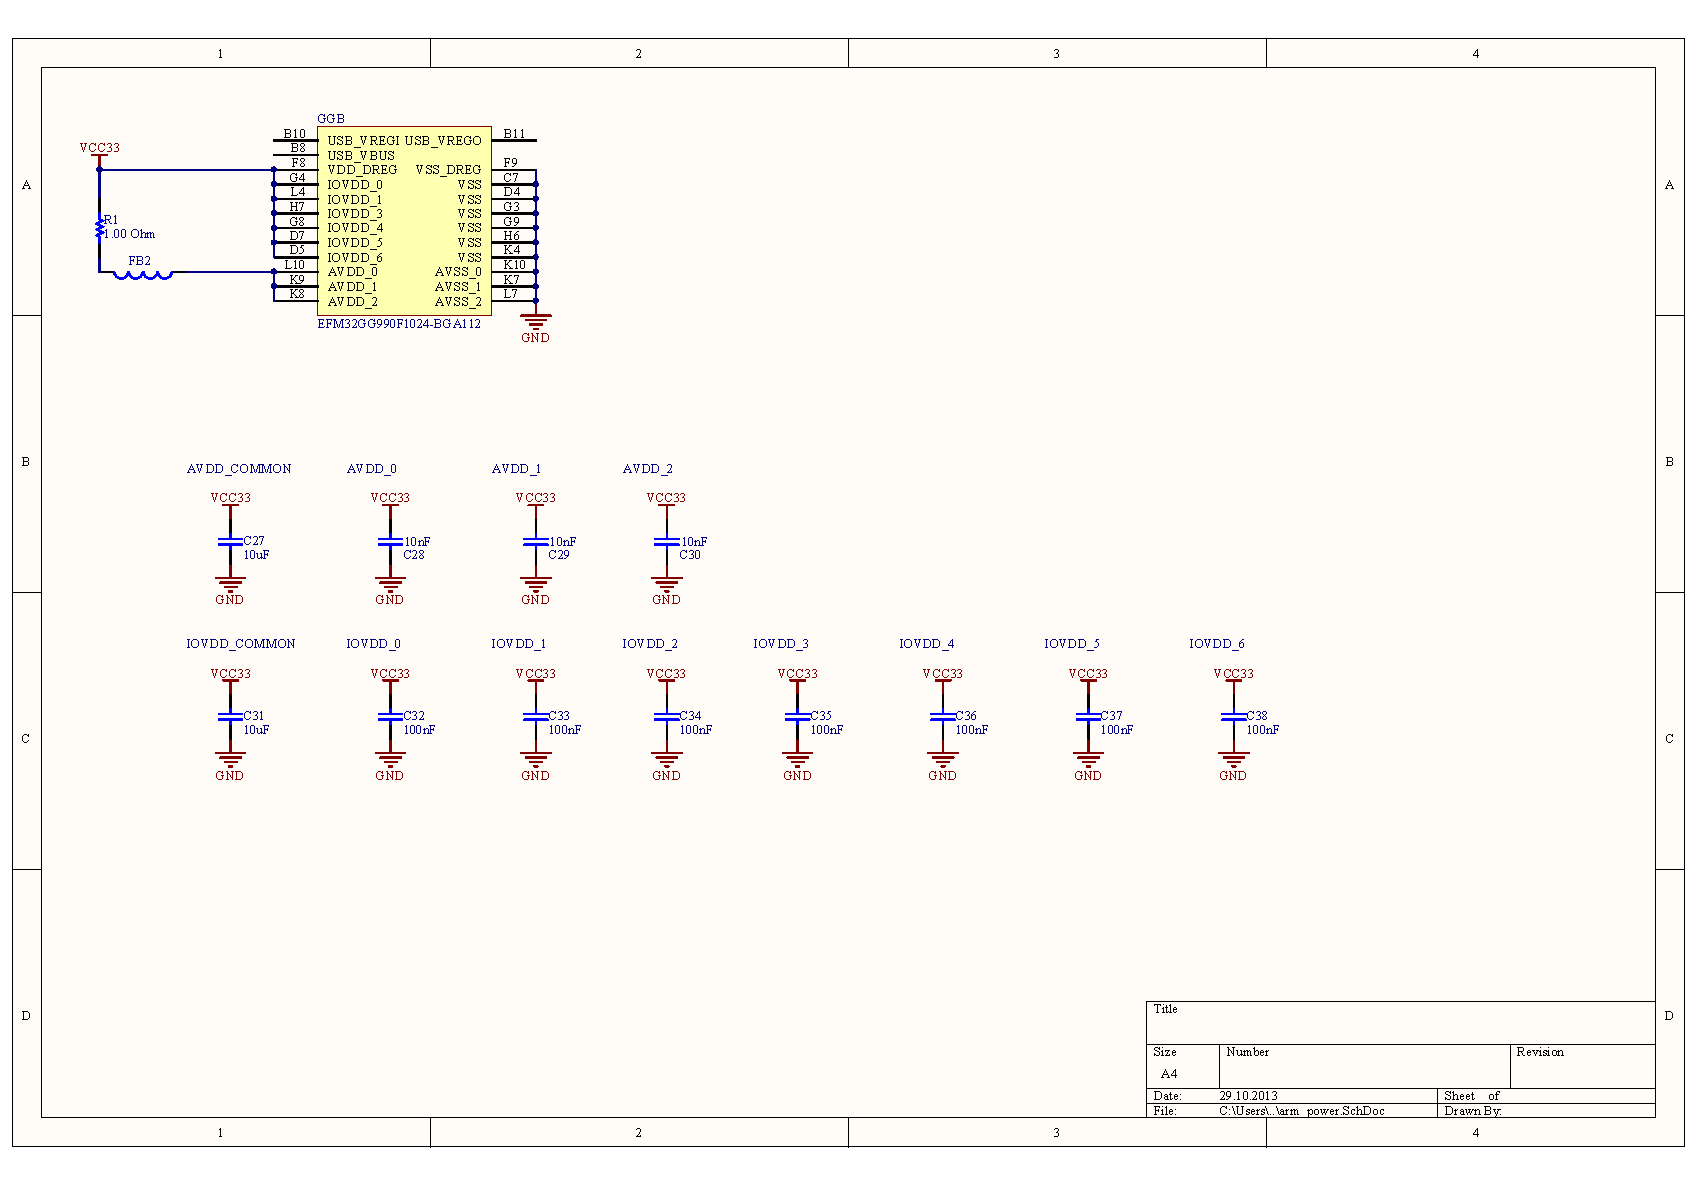
\includepdf[pages=-]{../pcb/take1/take1.pdf}
% !TEX root = ../../report.tex
\section{Components}

The PCB group was eager to learn how modern PCB production is done, using the
same tools and technologies as the industry. Thus, our choice of components was
strongly driven by a smaller is better mindset. The use of BGA packages (for
the MCU and FPGA) was already given from the resources we had available and the
fact that Odd Rune Lykkebo had experience baking these.

We used 0805 surface-mount components as much as possible, because they were the
smallest packages we could comfortably solder. This not only lowered the
production cost, but also allowed us to place components on both sides of the
board, and consequently minimizing the size.

{\bf USB-UART}
\begin{itemize}
  \item FTDI FT232RL - USB-UART converter
  \item 1x 4k7 and 1x 10k
  \item 3x 100nF and 1x 4.7uF
  \item USB3140-30-0170-1-C USB Micro B connector 
\end{itemize}


  



	

\section{Layout}
% !TEX root = ../../../../report.tex

\subsubsection{Routing}

Almost everything was autorouted, with only a few exceptions. The power supply had to be done manually, as well as the fanout on the FPGA. The routes are visible in the last image of Appendix~\ref{apx:schematics}.
% !TEX root = ../../report.tex
\section{Layer Stack}

We had three primary voltage levels on the PCB -- 1.2V, 1.8V and 3.3V. To
minimize resistance in the power distribution system, we decided to dedicate a
layer on the PCB to be used as a shared power plane. Another plane was used for
common ground and covered the whole PCB (excluding non-grounded through-holes).
This is setup with a shared ground and split power plane is common practice for
modern PCB design.

As for the signal layers, the BGA packages we used had only 0.8 mm pitch between
its feets. This forced us to have more signal layers than we originally set out
for, to be able to fanout and escape the BGA packages. Using a QFP-like package
could probably have saved us some cost, but using BGA gave us a valuable
experience on modern PCB design.

We settled upon a total of 8 layers on the PCB.

% !TEX root = ../../../../report.tex
\subsubsection{Footprints}

Each component is associated with a schematic drawing and a footprint. Because certain components were not available in public libraries they had to be drawn from scratch. Below is a list of all custom drawings and footprints.

\begin{table}[h]
	\centering
	\begin{tabular}{|l l l|}
		\hline
		\textbf{Component} & \textbf{Footprint}  & \textbf{Schematic} \\
		\hline
		XP Power Switch-Mode Regulator & X & X \\
		Würth Electronics MicroSD & X & X \\
		Molex MicroUSB AB & X & X \\
		Lumberg 3.5mm audio jack & X & X \\
		Buttons & X & X \\
		DC-10B & X & X \\
		Texas Instruments Op amp & X & X \\
		Diodes INC. Linear regulator& X & X \\
		Cypress Semiconductor SRAM & X & X \\
		& X & X \\
		& X & X \\
		& X & X \\
		& X & X \\
		\hline
	\end{tabular}
	\caption{Custom footprints and schematics}
	\label{tab:footprints}
\end{table}

\todo{finish table}

